
% This is samplepaper.tex, a sample chapter demonstrating the
% LLNCS macro package for Springer Computer Science proceedings;
% Version 2.21 of 2022/01/12
%
\documentclass[runningheads]{llncs}
%
\usepackage[T1]{fontenc}
% T1 fonts will be used to generate the final print and online PDFs,
% so please use T1 fonts in your manuscript whenever possible.
% Other font encondings may result in incorrect characters.
%
\usepackage{graphicx}
% Used for displaying a sample figure. If possible, figure files should
% be included in EPS format.
%
% If you use the hyperref package, please uncomment the following two lines
% to display URLs in blue roman font according to Springer's eBook style:
%\usepackage{color}
%\renewcommand\UrlFont{\color{blue}\rmfamily}
%

\bibliographystyle{splncs04}% the mandatory bibstyle
\usepackage{booktabs}   %% For formal tables:
                        %% http://ctan.org/pkg/booktabs
\usepackage{subcaption} %% For complex figures with subfigures/subcaptions
                        %% http://ctan.org/pkg/subcaption



\usepackage{mathtools}
\usepackage{todonotes}
\usepackage{microtype}

\usepackage{complexity}
\usepackage{amsmath}

\usepackage{stmaryrd}
\usepackage{dsfont}



\usepackage{mathrsfs}
\usepackage{mathalpha}
\usepackage{amsmath}
\usepackage{amsfonts}


\usepackage{ textcomp } 

\usepackage{stmaryrd}
\usepackage{wrapfig}


%


\newcommand{\problemx}[3]{
	\vspace{0.2cm}
\par\noindent\underline{\sc#1}\par\nobreak\vskip.2\baselineskip
\begingroup\clubpenalty10000\widowpenalty10000
\setbox0\hbox{\bf INPUT:\ }\setbox1\hbox{\bf QUESTION:\ }
\dimen0=\wd0\ifnum\wd1>\dimen0\dimen0=\wd1\fi
\vskip-\parskip\noindent
\hbox to\dimen0{\box0\hfil}\hangindent\dimen0\hangafter1\ignorespaces#2\par
\vskip-\parskip\noindent
\hbox to\dimen0{\box1\hfil}\hangindent\dimen0\hangafter1\ignorespaces#3\par
\endgroup
	\vspace{-0.2cm}
}

\newcounter{claimcounter}
\setcounter{claimcounter}{0}
\newtheorem{subclaim}{Subclaim}{}
\newtheorem{fact}{Fact}{}



\makeatletter



\renewcommand{\poly}{\mathrm{poly}}


\newcommand{\alain}[1]{\todo[inline,color=red!20]{{\bf AF:} #1}}
\newcommand{\mathieu}[1]{\todo[inline,color=blue!20]{{\bf MH:} #1}}



\newcommand{\pred}{\textsf{pred}}
\newcommand{\post}{\textsf{post}}


\newcommand{\Bad}{\textsf{Bad}}
\newcommand{\Safe}{\textsf{Safe}}


\begin{document}
%
\title{Resilience and Home-Space for WSTS \thanks{This work was partly done while the author was supported by the Agence Nationale de la Recherche grant BraVAS (ANR-17-CE40-0028).}} 
%
%\titlerunning{Abbreviated paper title}
% If the paper title is too long for the running head, you can set
% an abbreviated paper title here
%
\author{Alain Finkel\inst{1,2,3} \and Mathieu Hilaire\inst{1,3}}
% This research has been supported by ANR programme BraVAS (ANR-17-CE40-0028).
%
\authorrunning{A. Finkel, M. Hilaire.}
% First names are abbreviated in the running head.
% If there are more than two authors, 'et al.' is used.
%
\institute{Université Paris-Saclay, CNRS, ENS Paris-Saclay, LMF, Gif-sur-Yvette, France %\email{hilaire@lsv.fr}
\and
Institut Universitaire de France \and Agence Nationale de la Recherche grant BraVAS (ANR-17-CE40-0028)
}
%
\maketitle              % typeset the header of the contribution
%





\begin{abstract}
\noindent
Resilience of unperfect systems is a key property for improving safety by insuring that if a system could go into a bad state then it can also leave this bad state and reach a safe state.
We consider six types of resilience (one of them is the home-space property) defined by an upward closed set Safe  ($\Safe=\uparrow \Safe$) or downward-closed set ($\Safe=\downarrow \Safe$) (Bad is generally the complementary of Safe) and by the existence of a bound $k$ on the length of minimal runs starting from Bad and reaching Safe. We study the decidability of each type of resilience for two kinds of models: WSTS and VASS. We first show that most of all resilience problems are undecidable for WSTS with strong compatibility (and with effective pred-basis). Then we prove the decidability of resilience for completion-post-effective $\omega^2$-WSTS with strong compatibility (almost all known WSTS are in this class) and $\Safe = \uparrow \Safe$. Moreover, some resilience properties are decidable for three other classes of WSTS : (1) WSTS with effective 
$\uparrow$ $\post^*$ basis and $\Safe=\uparrow \Safe$ ; (2) ideal-effective WSTS with downward and upward compatibilities ; and (3) ideal-effective downward-compatible WSTS with $\Safe=\downarrow \Safe$. Finally, we study the resilience for VASS with semi-linear subsets Bad and Safe and for variations of VASS (lossy counter machines, integer VASS and continuous VASS); most of the resilience properties are shown decidable.
\end{abstract}

\keywords{Verification, Resilience, Home-Space, Well-structured transition systems, Vector addition system with states}



\newcommand{\LCM}{\mathsf{LCM}}
\newcommand{\LOGSPACE}{\mathsf{LOGSPACE}}
\newcommand{\MSO}{\mathsf{MSO}}
\newcommand{\SO}{\mathsf{SO}}

 \newcommand{\N}{\mathds{N}}



\section{Introduction}\label{section introduction}


{\bf Context.} 
Resilience is a key notion for improving safety of unperfect systems and resilience engineering is a paradigm for safety management that focuses on systems coping with complexity and balancing productivity with safety~\cite{challenges}. Some systems are subjects at frequent intervals to accidents, attacks or changes. Think for instance of a supply chain, or an airport’s air trafic control. In such cases, a question that arises is that of whether the system can return to its normal (safe) behavior after an accident or attack
pushed it towards some kind of ‘error state’ and, if it can, whether it can perform the return in a satisfactory timeframe. 


{\bf Home-spaces}
 In 1986, Memmi and Vautherin introduced the notion of home-space~\cite{DBLP:conf/ac/MemmiV86} for a system $\mathscr{S} = (S,\rightarrow )$ with an initial state $s_0$ : a subset $H \subseteq S$ is an \emph{home-space}  if 
$\post^*(s_0) \subseteq \pred^*(H)$. If the home-space contains a single element, this element is an {\em home-state}.
It could be easily generalized for two subsets $X,H$ and we say that $H$ is an \emph{home-space for $X$} if $\post^*(X) \subseteq \pred^*(H)$. In 1989, de Frutos Escrig and Johnen proved that the home-space problem (for $X$ a singleton and $H$ a finite union of linear sets with the same period) was decidable for VASS (only published as an internal report). In 2023, Jancar and Leroux proved the decidability of the (complete) semilinear home-space problem ($X$ and $H$ are both semilinear)  in VASS \cite{DBLP:journals/corr/abs-2207-02697}.
%%%%%

{\bf Resiliences.}  
The (general) resilience property for a transition system $\mathscr{S} = (S,\rightarrow )$ and a subset of states $\Safe \subseteq S$ consists of the following: $\mathscr{S}$ is {\em $\Safe$-resilient} if
$S \subseteq \pred^*(\Safe)$. It 
can be stated as an home-space problem : $\mathscr{S}$ is $\Safe$-resilient if $\post^*(S) \subseteq \pred^*(\Safe)$.
Similarly, $\mathscr{S}$ is $\Safe$-state-resilient for an initial state $s_0$ if  
$\post^*(s_0) \subseteq \pred^*(\Safe)$.
We will study three decidability questions for each of type of resilience.
The resilience problem is to decide whether a transition system $\mathscr{S} = (S,\rightarrow )$ is $\Safe$-resilient (for a given subset of states $\Safe \subseteq S$).
The resilience problem could be easily generalized for two subsets $\Bad$ and $\Safe$ by asking
whether $\Bad \subseteq \pred^*(\Safe)$.
The $k$-resilience problem is to decide whether $S \subseteq \pred^{\leq k}(\Safe)$ (for a given $k$) and 
the bounded resilience problem is to decide whether there exists an $k$ such that $\mathscr{S}$ is $\Safe$-$k$-resilient. We adapt these three definitions to state-resilience.


{\bf State of the art.}
In 2016, Prasad and Zuck introduced in  \cite{DBLP:journals/corr/PrasadZ16} interesting definitions and results (without detailed proofs) about resilience in the framework of process algebra. They built the composition of the process and its adversary as a transition system and they gave conditions that insure that the composed transition system is an effective WSTS with both upward and reflexive downward compatibilities (and some other technical conditions). In this framework and under these hypotheses, resilience reduces to coverability which is decidable on WSTS. 
%%%%%%%%%

In 2021, \"Ozkan and Würdemann  \cite{DBLP:journals/corr/abs-2108-00889} and \"Ozkan \cite{DBLP:conf/gg/Ozkan22}, in 2022, proved the decidability of the bounded state-resilience problem and the $k$-state-resilience problem for WSTS  with strong compatibility and with the supplementary (strong) hypothesis that there exists an algorithm that computes a finite basis of $\uparrow \post^*(s)$ for all state $s$ (called effective 
$\uparrow$ $\post^*$ basis) and with $\Safe=\uparrow \Safe$ and $\Bad$ downward-closed.


Remark that the reflexive downward compatibility (of an effective WSTS) hypothesis in  \cite{DBLP:journals/corr/PrasadZ16} implies the existence of an algorithm that computes a finite basis of $\uparrow \post^*(s)$ for all state $s$; this provides a way to use \cite{DBLP:journals/corr/abs-2108-00889} for proving the announced result by Prasad and Zuck.
However, neither Prasad \& Zuck nor \"Ozkan \& Würdemann established the strong relation between resilience and the home-space property.
%%%%%%%%%
%




\noindent
{\bf Our contributions}
\begin{itemize}
\item Surprinsingly, the general undecidability statements about resilience were not known neither proved. We show that resilience and { State-resilience} problems are both undecidable for WSTS with strong compatibility. 
Moreover, {State-resilience},
{Bounded-state-resilience} and
{$k$-state-resilience}
are undecidable for strongly upward-compatible WSTS with effective pred-basis
when
$\Safe=\uparrow \Safe$. We made a reduction of zero-reachability in reset-VASS to {\ State-resilience} in reset-VASS.


\item The three resilience problems are decidable for completion-post-effective $\omega^2$-WSTS with strong compatibility and $\Safe = \uparrow \Safe$.


\item The resilience problem is decidable for ideal-effective WSTS with 
$\Safe=\downarrow \Safe$
and
the additional hypothesis that
for all downward-closed set $D \subseteq S$, the set $\pred^*(D)$ is downward-closed.
%
%%%

\item We generalize the main theorem of \cite{DBLP:journals/corr/abs-2108-00889,DBLP:conf/gg/Ozkan22} by relaxing the strong compatibility hypothesis.
We also show that removing the effective 
$\uparrow$ $\post^*$ basis hypothesis leads to undecidability. We extend and prove the main result in  \cite{DBLP:journals/corr/PrasadZ16} : the three state-resilience problems are decidable for ideal-effective WSTS with downward and upward compatibilities ({ $k$-state-resilience} and { bounded-state-resilience} are decidable for ideal-effective WSTS with strong downward compatibility).
%

\item We study the resilience problems for VASS and variations of VASS where most of the resilience problems are shown decidable.
\end{itemize}


 \begin{center}
	\begin{figure}
			\hspace{0.8cm}
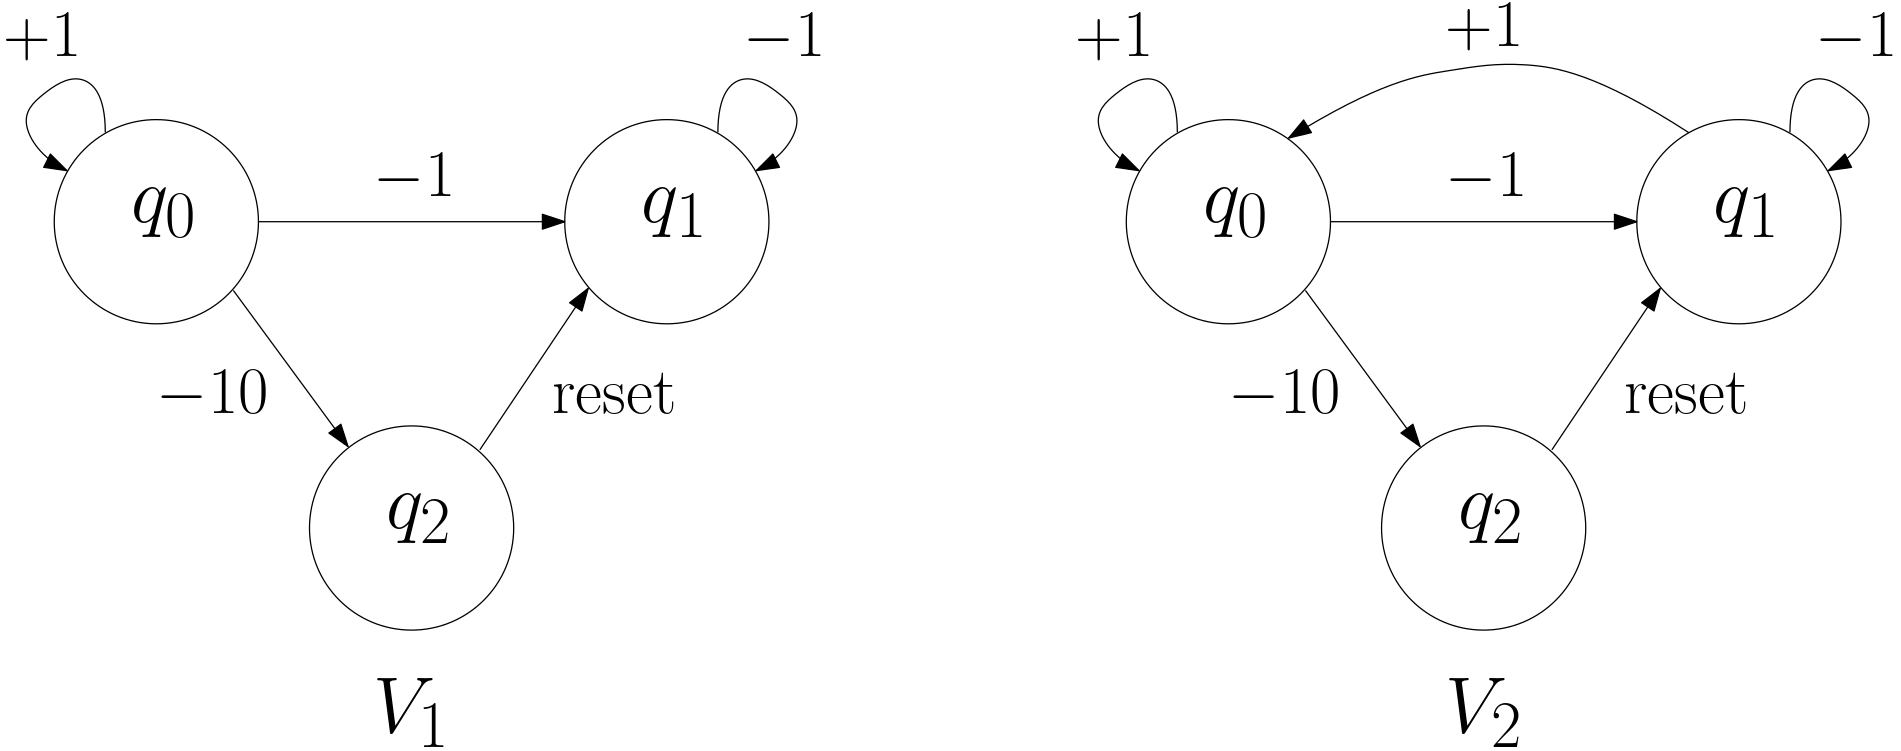
\includegraphics[width=0.75\textwidth]{FigureCD}
	\caption{Two reset-VASS with three control-states and one counter.}
					\label{r-V}
	\end{figure}
\end{center}

\begin{example}\label{Example}
{(\bf Reset-VASS example).}
Consider the 
 reset-VASS $V_1$ from Figure~\ref{r-V}.
Consider first $\Safe = \{q_0(n) \mid n \in \N\}$; In this case,  {resilience}, 
{$k$-resilience} and {bounded resilience} are not satisfied: there is no  way back from $q_2$ or $q_1$ to $q_0$. Consider now $\Safe = \{q_1(0)\} $; then {resilience} hold: it is possible to reach $q_1(0)$ from any configuration of $V_1$. However, {bounded resilience} does not hold, since, for all $n\in \N$, from $q_1(n)$, there is no path of length less than $n$ towards $q_1(0)$. Consider now the 
 reset-VASS $V_2$, which is $V_1$ plus an $+1$ transition from $q_1$ back to $q_0$. In $V_2$, {bounded resilience} hold, since $6$-resilience hold. 
Indeed, from any configuration with value of the counter bigger than $9$, it is possible to reach $q_2$ in two steps or less, then use the (unique) reset transition. From $q_1(n)$ or $q_0(n)$ with $n \in \{1, 2, 3, 4, 5, 6\}$ it is possible to reach $q_1(0)$ in $6$ steps or less. From 
$q_1(n)$ or $q_0(n)$ with $n \in \{7,8\}$ it is possible to reach $q_0(10)$ in $3$ steps or less, from which $q_1(0)$ is reachable in $2$ steps. 
\end{example}

Hence we can see how adding transitions can 
turn a system that is not bounded resilient into one that is. 





\section{Well-structured transition systems and VASS}\label{section definitions}



\noindent
 A {\em transition system} is a pair $\mathscr{S} = (S,\rightarrow )$ where $S$ is a set of 
 {\em states (or configurations)} and  
 $ {\rightarrow} \subseteq S \times S$ is a
 binary relation 
 on
 the set of states, denoted as the set of {\em transitions}. 
%
We write $s \rightarrow s'$ to denote $ (s,s') \in  {\rightarrow} $.
We write $\rightarrow^{k}$, $\rightarrow^{+}$, $\rightarrow^{=}$, $\rightarrow^{*}$
for the $k$-step iteration of $\rightarrow$, its transitive closure, its reflexive closure, its reflexive and transitive closure.
Let $X,Y \subseteq S$ and $k \in \mathbb{N}$; we denote $X \longrightarrow^{*} Y$ (resp. $X \longrightarrow^{\leq k} Y$) if from all states $x \in X$ there exists a path (resp. of length smaller than $k$) that reaches a state $y \in Y$.
\noindent
The set of {\em (immediate) successors} of a state $s \in S$ is defined as 
 $\post(s) = \{ s' \in S \mid  ~ s \xrightarrow{} s'\}$. 
The set of {\em (immediate) predecessors} of a state $s \in S$ is defined as
 $\pred(s) = \{ s' \in S \mid  ~ s' \xrightarrow{} s\}$. 
By iterating $\pred$ and $\post$ we obtain  
$\post^n(s) = \{ s' \in S \mid  ~ s \xrightarrow{}^n s'\}$
and
$\pred^n(s) = \{ s' \in S \mid  ~ s' \xrightarrow{}^n s\}$.
However, we are generally more interested in
$\post^{\leq n}(s) = \bigcup_{1 \leq i \leq n} \post^i(s)$, $\post^*(s)= \bigcup_{1 \leq i} \post^i(s)$
and
$\pred^{\leq n}(s) = \bigcup_{1 \leq i \leq n} \pred^i(s)$ and $\pred^*(s) = \bigcup_{1 \leq i} \pred^i(s)$. 
The {\em reachability problem} asks, given a transition system $\mathscr{S} = (S, \to)$, two states $s, t \in S$, whether $s \to^* t$. 

%


A {\em quasi-ordering} (a qo) is any reflexive and transitive relation $\leq$ over some set $X$ and we often write $(X,\leq)$. 
Given $(X,\leq)$ a quasi-ordering, an {\em upward-closed set} is any set $U \subseteq X$ such that if $y \geq x$ and $x \in U$ then $y \in U $.
A {\em downward-closed set} is any set $D \subseteq X$ such that if $y \leq x$ and $x \in D$ then $y \in D $. 
It is an {\em ideal } if it is also {\em directed}, i.e. it is nonempty and for every $a,b \in D$, there exists $c \in D$ such that $a \leq c$ and $b \leq c$.
To any subset $A \subseteq X$, we may associate
its {\em upward-closure},
 $\uparrow A = \{x \in X \mid \exists a \in A ~ y \geq a\}$
 and its 
 {\em downward-closure},
 $\downarrow A = \{x \in X \mid \exists a \in A ~ y \leq a\}$. 
We abbreviate $\uparrow \{x\}$ (resp. $\downarrow \{x\}$)
as $\uparrow x$ (resp. $\downarrow x$).
%
A {\em basis} of an upward-closed set $I$ is a set $I_b$ such that $I = \uparrow I_b$. 


 A {\em well-quasi-ordering} (wqo) is any quasi-ordering $(X,\leq)$ such that, for any infinite sequence $x_0, x_1, x_2, ...$ in $X$, there exist indexes $i \leq j$ with $x_i \leq  x_j$.
%
%
%
Wqo admits many other equivalent formulations. 
%
%
As an example, $(\N^d, \leq)$, the set of vectors of $d$ natural numbers (where $d$ is finite) with component-wise order is a wqo.
%
Quasi-orderings that have no 
infinite subset of mutually incomparable elements (antichains)
 enjoy a similar \emph{finite decomposition} property than wqo: every downward-closed subset $D \subseteq X$ can be decomposed into a \emph{finite} set of ideals $J_1, J_2,..., J_n$ such that $D = \downarrow (J_1 \cup J_2 \cup..\cup J_n)$.
%
%
In what follows, a downward-closed set $D$ is represented by its finite set of ideals (or by the minimal elements of its upward-closed complement), and an upward-closed set $U$ is represented by its finite set of minimal elements. \\

\noindent
Let us now recall the (most general) definition of well-structured transition systems.
\begin{definition}\cite{DBLP:journals/iandc/Finkel90,DBLP:journals/tcs/FinkelS01}
A {\em well-structured transition system} (WSTS)  $\mathscr{S}=(S, \rightarrow, \leq)$
is a transition system $(S, \rightarrow)$
equipped with a wqo ${\leq} \subseteq S \times S$ such that   
the transition relation $ \rightarrow$ is (upward) compatible with $\leq$, i.e., for all 
$s_1, t_1 , s_2 \in S$
	with $s_1 \leq s_2$  and $s_1 \rightarrow t_1$, there exists 
	$t_2 \in S$ with 
	$t_1 \leq t_2$ and $s_2 \rightarrow^{*} t_2$.
\end{definition}

We say that a WSTS $\mathscr{S}$ has \emph{strong (upward) compatibility} when moreover for all 
$s_1, t_1 , s_2 \in S$
	with $s_1 \leq s_2$  and $s_1 \rightarrow t_1$, there exists 
	$t_2 \in S$ with 
	$t_1 \leq t_2$ and $s_2 \rightarrow t_2$.

Several families of formal models of processes give rise to WSTSs in a natural way, e.g. Petri nets when inclusion between markings is used as the well-ordering and lossy channel systems with the subword ordering. 


\noindent
{\bf On effectivity}
Let a WSTS $\mathscr{S}=(S, \rightarrow, \leq)$. We say that $\mathscr{S}$ is {\em effective} if there exists a pair of algorithms
($M_\rightarrow$, $M_\leq$) operating on $\N \times \N$ such that
$ M_\rightarrow$ computes the transition relation “$\rightarrow$” and 
$M_\leq$ the ordering relation “$\leq$”.
We say that $\mathscr{S}$ is {\em post-effective} if it is effective, and if there
exists an algorithm that computes $|\post(x)| \in \N \cup \{\infty\}$ 
on input $x$, with $x \in X_i $. 
We say that $\mathscr{S}$ has {\em effective pred-basis} \cite{DBLP:journals/tcs/FinkelS01,DBLP:journals/iandc/AbdullaCJT00} if there exists an algorithm accepting
any state $s \in S$ and returning $pb(s)$, a finite basis of $\uparrow \pred(\uparrow s)$.
%
We say that $\mathscr{S}$
is {\em ideal-effective} \cite{BFM-ic17} if (1) the function mapping the encoding of a configuration $s$
to the encoding of the ideal $\downarrow s$ is computable; (2) inclusion of ideals is decidable; (3) the downward closure $\downarrow \post(I)$ expressed as a finite union of ideals is computable from the ideal $I$.
%

Now, we may recall a simple condition that insures that a finite basis of $\pred^*(\uparrow s )$ is computable for every $s \in S$.
We will use the following property: if $\mathscr{S}$ is a WSTS with strong compatibility and $U \subseteq S$ is upward-closed, then $\pred(U )$, $\pred^k(U )$ with $k\geq0$, and $\pred^*(U )$ are all upward-closed \cite{DBLP:journals/tcs/FinkelS01}.
For a WSTS $\mathscr{S}=(S, \rightarrow, \leq)$ and an upward-closed set $U  \subseteq S$, let us study the convergence of the sequence defined by $U_0=U$ and $U_k= U_{k-1} \cup \pred(U_{k-1})$ for $k \geq 1$. When $\mathscr{S}$ has strong compatibility, the sets $U_k$ are upward-closed and $U_k \subseteq U_{k+1}$ so we know that the sequence $(U_k)_k$ converges. Let us define the \emph{index} of convergence of the sequence $U_k$ as the smallest $k_0$ s.t. $U_k = U_{k_0}$ for all $k \geq k_0$. We may compute $k_0$ and we then have:  $\pred^*(U) = U_{k_0}$. 
With the effective pred-basis hypothesis, we obtain:

\begin{theorem}\cite{DBLP:journals/tcs/FinkelS01,DBLP:journals/iandc/AbdullaCJT00}
A finite basis of $ \pred^*(U)$ is computable for any effective WSTS $\mathscr{S}=(S, \rightarrow, \leq)$ with effective pred-basis and any upward-closed set $U \subseteq S$ given with its finite basis $B_U$. Hence coverability is decidable.
\end{theorem}

With the ideal-effective hypothesis, we obtain the decidability of coverability for a class of ordered transition systems larger than WSTS.

\begin{theorem}\cite{BFM-ic17}
Coverability is decidable for any ideal-effective ordered upward-compatible transition system $\mathscr{S}=(S, \rightarrow, \leq)$ where $\leq$ is without infinite antichains.
\end{theorem}




Let us recall the  definition of vector addition system with (control-)states. 
 \begin{definition} 
A {\em vector addition system with states (VASS)} in dimension $d$ ($d$-VASS for short) is a finite $\mathds{Z}^d$-labeled directed graph $V = (Q,T)$, where $Q$ is the set of {\em control-states}, and $T \subseteq Q \times \mathds{Z}^d \times Q$ is the set of {\em control-transitions}. 
 \end{definition} 
%
Subsetquently, $Q \times \N^d$ is the set of configurations of the transition system associated with a $d$-VASS $V$.
For all configurations $p(\textbf{u}), q(\textbf{v}) \in Q \times \N^d$ and for every control-transition $t = (p, \textbf{z}, q)$, we write $p(\textbf{u}) \xrightarrow{t} q(\textbf{v})$ whenever $\textbf{v} = \textbf{u} + \textbf{z} \geq \textbf{0}$
%
When in the context of a $d$-VASS, we denote $0^d$ by $\textbf{0}$.

A {\em vector addition system (VAS)} in dimension $d$ ($d$-VAS for short) is a $d$-VASS where the set of control-states is a singleton; hence it can be only defined by $T$.





\section{Resilience for WSTS}



In a transition system $\mathscr{S}=(S,\rightarrow)$, we consider a subset of states $\Safe \subseteq S$, and its complement, $\Bad$.
The \emph{resilience problem} (resp. the \emph{$k$-resilience problem}) for $(\mathscr{S},\Safe)$ is to decide whether from \emph{any} state in 
$S$, \emph{there exists} a path (resp. a path of length smaller than or equal to $k$) that reaches a state in $\Safe$. Resilience is then the Home-Space problem (defined in the introduction) for the set $\Safe$. We use the notation 
$S \longrightarrow^{*} \Safe$ (resp. $S \longrightarrow^{\leq k} \Safe$)
 for 
$\forall x \in S, \exists y \in \Safe$ 
 such that $x \longrightarrow^{*} y$ 
  (resp.  $\forall x \in S, \exists y \in \Safe$ such that $x \longrightarrow^{\leq k} y$).
  In our framework, $\Safe \subseteq S$  is possibly infinite but  must admit a computable finite representation : for example, downward-closed sets and upward-closed sets in wqo and semilinear sets in $\mathbb{N}^d$ have finite representations. 





Let us formalize three resilience problems.


\problemx{Resilience (RP)}
{A transition system $\mathscr{S}=(S,\rightarrow)$ and a set $\Safe \subseteq S$.}
{$S \longrightarrow^{*} \Safe$ ?\newline}



\problemx{$k$-resilience (kRP)}
{A transition system $\mathscr{S}=(S,\rightarrow), k \in \mathbb{N}$ and a sets $\Safe \subseteq S$.}
{$S \longrightarrow^{\leq k} \Safe$ ?\newline}

\problemx{Bounded resilience (BRP)}
{A transition system $\mathscr{S}=(S,\rightarrow)$ and a set $\Safe \subseteq S$.}
{$\exists k \geq 0$ such that {$S \longrightarrow^{\leq k} \Safe$ ?\newline}}


  
These three resilience problems are decidable for finite transition systems but undecidable for (general) infinite-state transition systems. So we restrict our framework to the class of infinite-state WSTS. Since most of decidable properties in WSTS rely on the computation of upward or downward-closed sets \cite{DBLP:journals/iandc/AbdullaCJT00,DBLP:journals/tcs/FinkelS01}, we consider upward-closed or downward-closed sets $\Safe$% and $\Bad$
. Since $\Safe \subseteq \pred^*(\Safe)$, one only need to decide whether 
the complement of $\Safe$ is in $\pred^*(\Safe)$. From now on, we use $\Bad$ to denote the complement of $\Safe$.
In \cite{DBLP:journals/corr/abs-2108-00889}, the authors considered that $\Safe$ is upward-closed.  



{\bf Related problems.} 
Resilience and the home-space problem are also linked to the 
model-checking of basic reachability and safety formulae. 
In particular~\cite{DBLP:conf/rp/Schnoebelen10} shows that the ``from-all'' formula $\forall s \in X~ \exists t \in Y~ s \to^* t$
is decidable for Lossy Counter Machine (LCM)
when $X$ and $Y$ are semi-linear sets.
Other decidable formulae include ``one-to-one'' ($\exists s \in  X ~ \exists t \in  Y ~ s \to^* 
 t$), and ``all-to-same'' ($\exists t \in  Y ~ \forall s \in  X ~ s \to^*  t$),
whereas ``one-to-all'' ($\exists s \in  X ~ \forall t \in  Y ~ s \to^*  t$), 
``all-to-all'' ($\forall s \in  X ~ \forall t \in  Y ~ s \to^*  t$)
  and ``to-all'' ($\forall t \in  Y  ~ \exists s \in  X ~ s \to^*  t$) are undecidable (again, for LCM). 
  
  
  





\subsection{Case: $\Safe=\uparrow \Safe$.}\label{safe-up}

We start with the case $\Safe=\uparrow \Safe$, hence $\Bad=\downarrow \Bad$. 
Resilience can be viewed as a generalizeation
 of coverability, as
it asks whether for \emph{every} element of $\Bad$ it is possible to cover an element of the basis of $\Safe$.


Let us recall that the \emph{completion}  \cite{BFM-ic17} of a WSTS $\mathscr{S}=(S,\rightarrow, \leq)$ is the associated ordered transition system $\hat{\mathscr{S}}=(Ideals(S),\rightarrow, \subseteq)$ where states of $\hat{\mathscr{S}}$ are ideals of $S$ and $I \rightarrow J$ if $J$ belongs to the finite ideal decomposition of $\downarrow \post_{\mathscr{S}}(I)$. The completion is always finitely branching but it is not necessarly WSTS since $\subseteq$ is not necessarly a wqo. $\hat{\mathscr{S}}$ is WSTS iff $\mathscr{S}=(S,\rightarrow, \leq)$ is $\omega^2$-WSTS (intuitively speaking, $(S,\leq)$ must not contain the Rado set). 
A WSTS $\mathscr{S}=(S,\rightarrow,\leq)$ is {\em completion-post-effective} if
it is post-effective, and there exists a Turing Machine $M_\downarrow$ that computes, on input $s \in S$, 
 $\downarrow s$, and some Turing Machine $M_{\uparrow^C}$ that computes, on input
 $\{s_1, s_2, \ldots, s_m\} \in S^m$, 
 the ideal decomposition of $S \setminus \uparrow \{ s_1, s_2, \ldots, s_m\}$.
Coverability is shown decidable  [Theorem 44] in \cite{BFM-ic17} for completion-post-effective $\omega^2$-WSTS (we don't need the pred-basis hypothesis).

Let us recall two other results in \cite{BFM-ic17}. Proposition 30 establishes a strong relation between the runs of a WSTS $\mathscr{S}=(S,\rightarrow, \leq)$ and the runs of its completion $\hat{\mathscr{S}}$. It states that if $x \xrightarrow{k} y$ in $\mathscr{S}$ then for every ideal $I \supseteq \downarrow x$, there exists an ideal $J \supseteq \downarrow y$ such that $I \xrightarrow{k} J$ in $\hat{\mathscr{S}}$. Proposition 29 establishes that if $I \xrightarrow{k} J$ in $\hat{\mathscr{S}}$ then for every $y \in J$, there exists $x \in I$ and $y' \geq y$ such that $x \xrightarrow{k'} y'$ in $\mathscr{S}$. Moreover, if $\mathscr{S}$ has transitive compatibility then $k’ \geq k$; if $\mathscr{S}$ has strong compatibility then $k’ = k$.
%





%
\begin{theorem}\label{down-up}
Let $\mathscr{S}=(S,\rightarrow, \leq)$ be a completion-post-effective $\omega^2$-WSTS with strong compatibility and a set $\Safe = \uparrow \Safe$.
{\sc Resilience}, {\sc Bounded resilience} 
and {\sc $k$-resilience} are decidable.
\end{theorem}

\begin{proof}
Let  $\{b_1,b_2,...,b_m\}$ be the (unique) minimal basis of $\Safe$ and  $\{J_1, J_2,...,J_n\}$ be the ideal decomposition of $\Bad$.
The resilience problem can be reduced to the following infinite number of instances of the coverability problem in $\mathscr{S}$: for all $x \in \Bad$ does there exist an $j$ such that $b_j$ is coverable from $x$. Let us show how this infinite set of coverability questions can be reduced to a \emph{finite} set of coverability questions in the completion $\hat{\mathscr{S}}=(Ideals(S),\rightarrow, \subseteq)$ of $\mathscr{S}=(S,\rightarrow, \leq)$. 


Let us prove that $b_j$ is coverable from $x$ in $\mathscr{S}$ if and only if $\downarrow b_j$ is coverable (for inclusion) from $\downarrow x$ in $\hat{\mathscr{S}}$.
%
Suppose that $b_j$ is coverable from $x$ then there exists a run $x \xrightarrow{k} y \geq b_j$. From Proposition 30, there exist an ideal $J$ and a run $\downarrow x \xrightarrow{k} J$ where $J \supseteq \downarrow y \supseteq \downarrow b_j$ in $\hat{\mathscr{S}}$, hence $\downarrow b_j$ is covered from $\downarrow x$.
Conversely, if $I \xrightarrow{k} J$ in $\hat{\mathscr{S}}$ with $\downarrow b_j \subseteq J$ then 
%	for every $y \in J$, 
there exists $x \in I$ and $y' \geq b_j$ such that $x \xrightarrow{k} y'  \geq b_j$ in $\mathscr{S}$ and then $b_j$ is coverable from $x$ in $\mathscr{S}$.

Hence we obtain: $\mathscr{S}$ is resilient iff for all $i=1,..,n$ and $j= 1,..m$, $\downarrow b_j$ is coverable from ideal $J_i$ in $\hat{\mathscr{S}}$.
%
Let us denote by $k_{i,j}$ the length of a covering sequence that covers $\downarrow b_j$ from $J_i$ in $\hat{\mathscr{S}}$ and let $k_{i,j}\stackrel{\text{def}}{=}\infty$ if $\downarrow b_j$ is not coverable from $J_i$. Let us now define $K_{\mathscr{S}}(\Safe)=\max(k_{i,j} \mid i=1,..,n$ and $j= 1,..m$).
%

%
We now have $\mathscr{S}$ is resilient iff $K_{\mathscr{S}}(\Safe)$ is finite iff $\mathscr{S}$ is $K_{\mathscr{S}}(\Safe)$-resilient with $K_{\mathscr{S}}(\Safe)$ finite.

This implies that resilience and bounded resilience are equivalent to coverability.
Since coverability is decidable for completion-post-effective $\omega^2$-WSTS, we deduce that both the 
  resilience problem and the bounded resilience problem are decidable.



Let us now show that the $k$-resilience problem, with $k \in \mathbb{N}$, is also decidable.
Let us denote by $k'_{i,j}$ the \emph{minimal} length of a covering sequence that covers $\downarrow b_j$ from $J_i$ in $\hat{\mathscr{S}}$ if it exists and let $k'_{i,j}\stackrel{\text{def}}{=}\infty$ if $\downarrow b_j$ is not coverable from $J_i$. 
If $\downarrow b_j$ is coverable from $J_i$, we first compute an $k_{i,j}$, and then we compute $k'_{i,j}$ by iteratively checking whether there exists a sequence of length $0,1,...,k_{i,j}-1$ that covers $\downarrow b_j$ from $J_i$ until we find the minimal one which is necessarly smaller (or equal to) than $k_{i,j}$.

Let us now define $K'_{\mathscr{S}}(\Safe)=\max(k'_{i,j} \mid i=1,..,n$ and $j= 1,..m$) and we deduce that  $\mathscr{S}$ is $k$-resilient iff $k \geq K'_{\mathscr{S}}(\Safe)$. \qed
\end{proof}


Remark that the previous proof don't make use of the 
property that $\Bad$ is the complement of $\Safe$, simply using
$\Bad=\downarrow \Bad$ and $\Safe=\uparrow \Safe$, thus 
the above results still hold in the more general case where $\Bad$ and $\Safe$ are not complements of each others.


The completion-post-effective hypothesis is needed to decide {\sc Resilience}.
Indeed, consider the family $\{ f_j: \N^2 \to \N^2\}$ of 
increasing recursive functions from \cite{FMP-ic04} defined as

$ f_j(n,k) = \begin{dcases*} (n,0) & \text{ if } k=0 \text{ and } TM$_j$ \text{ runs for more than } n \text{ steps} \\
		(n,n+k) &\text{ otherwise,} \end{dcases*} $
		
	\noindent	
	where $TM_j$ is the $j$-th Turing machine (in a classical enumeration)
	which moreover begins
by writing the integer $j$ on its tape,	
	and consider additionnally the function $g : \N^2 \to \N^2$ defined by $g(n,k) = (n+1,k)$. 
	The
	transition system 
	$S_j = (\N^2, \{f_j, g\}, \leq)$ 
	is a WSTS
	and
	has the property that
	it is
	$\uparrow (1,1)$-resilient
	iff $TM_j$ halts on input $j$,
	since $(1,1)$ is coverable from $(0,0)$
	iff $TM_j$ halts on input $j$. 
	Hence there is no Turing machine which correctly determines 
	resilience and halts whenever its input is a
	WSTS.
Hence resilience for WSTS in general is undecidable.




\subsection{Case: $\Safe=\downarrow \Safe$.}\label{safe-down}


Let us now consider the case $\Safe=\downarrow \Safe$ hence $\Bad=\uparrow \Bad$.
It is of interest to note this case can be linked to the problem of mutual exclusion.
Indeed the well-known mutual exclusion property can be modelized, in a $d$-VASS with $d$ counters, by the property that a special counter $c_{mutex}$ must be bounded by $k \geq 1$ which counts the (maximal) number of processes that are allowed to be simultaneously in the critical section. Then, the set $\Safe =  \{c_{mutex} \leq k\} \times \mathbb{N}^{d-1}$ is downward-closed		and $\Bad =\{c_{mutex} \geq k+1\} \times  \mathbb{N}^{d-1} $ is the upward-closed complementary of $\Safe$. 


%
\begin{theorem}\label{up-down}
{\sc Resilience}  is decidable for ideal-effective WSTS with 
$\Safe=\downarrow \Safe$
and
the additional hypothesis that
for all downward-closed set $D \subseteq S$, the set $\pred^*(D)$ is downward-closed.
\end{theorem}

\begin{proof}
By hypothesis $\pred^*(\Safe)$ is downward-closed, since $\Safe$ is downward-closed.
The resilience problem can be reformulated as 
$\Bad \subseteq  \pred^*(\Safe)$.
Since $\mathscr{S}=(S,\rightarrow, \leq)$ is ideally effective, we can compute intersections of upward- or downward-closed 
 subsets.
Hence we can compute the intersection of
$\Bad$
and
$S \setminus \pred^*(\Safe)$,
which are both upward-closed.
Since
$\Bad \subseteq \pred^*(\Safe)$
can be reformulated as
$\Bad \cap (S \setminus \pred^*(\Safe)) = \emptyset$
the resilience problem is decidable. \qed
\end{proof}

Let us recall that a system $\mathscr{S}=(S,\rightarrow, \leq)$ is \emph{downward compatible} \cite{DBLP:journals/tcs/FinkelS01} if
for all $s_1, s_2, t_1 \in S$ with
$s_2 \leq s_1$ and $s_1 \to t_1$
there
exists $t_2 \in S$ with
$t_2 \leq t_1$ and $s_2 \to^* t_2$.

\begin{corollary}
{\sc Resilience} is decidable for ideal-effective downward-compatible WSTS with 
$\Safe=\downarrow \Safe$.
\end{corollary}

\begin{proof}


Let $D$ be a downward-closed subset of $S$
and let $x \in \downarrow \pred^*(D)$.
By downward closure, there exists
$y \in \pred^*(D)$ 
such that $x \leq y$.
By definition of $\pred^*(D)$ then there exists 
$d \in D$, $m\geq 0$ and $(a_i)_{0 \leq i \leq m+1} \in S^{m+2}$ such that
$y = a_0 \to a_1 \to a_2 \to \cdots \to a_m \to a_{m+1} = d$.

By downward compatibility $a_0 \to a_1$
implies that there exists $a'_1 \in S$ such that $a'_1 \leq a_1$ and
$x \to^* a'_1$.
More generally $a_i \to a_{i+1}$ and
$a'_i\leq a_i$ implies the existence of $a'_{i+1} \in S$ with $a'_{i+1} \leq a_{i+1}$ and
$a'_i \to^* a'_{i+1}$,
and, by induction,
 $x \to^* a'_1 \to^* \cdots \to^* a'_{m} \to^* a'_{m+1} = d'$
with $d' \leq d$.
Since
$d'$ 
belongs to $D$ by downward closure of $D$, $x \in \pred^*(D)$. \qed
\end{proof}


In the case
of a ideal-effective WSTS 
where
the additional hypothesis that
for all downward-closed set $D \subseteq S$, the set $\pred^*(D)$ is downward-closed
is not met,
the above construction
can provide a proof
of non-resilience
i.e. when
$\Bad \cap (S \setminus \downarrow\pred^*(\Safe)) \neq \emptyset$
then
$\Bad \not\subseteq \downarrow\pred^*(\Safe)$
and hence
$\Bad \not\subseteq \pred^*(\Safe)$.
When $\Bad \cap (S \setminus \downarrow\pred^*(\Safe)) = \emptyset$
however
it is not enough to conclude.



In the case
of a ideal-effective WSTS 
where the hypothesis that
{for all downward-closed set $D \subseteq S$, the set $\pred^*(D)$ is downward-closed}
is not met, the problem is undecidable.
 Indeed, it is 
undecidable for reset-VAS whether zero (the vector containing only zeroes, also denoted~$ \textbf{0}$) is a home-state for $\N^d \setminus \textbf{0}$, where it is a particular case of resilience with $\Safe = \downarrow \textbf{0}$. This stems from the fact that it is undecidable for Minsky machines with more than one counter, whether zero is a home-state.  




Home-space is undecidable for Minsky machine with at least $3$ counters, since it is undecidable in the particular case where $H$ is a singleton.
This stems from the fact $2$-counter Minsky machine termination is undecidable~\cite{Min61,Min67}.
From a $2$-counter Minsky machine $M$, one can construct a $3$-counter Minsky machine $M'$ 
such that machine $M$ terminates for all inputs iff machine $M'$ can reach $(0,0,0)$ from any input with at least $1$ on its third counter. We build $M'$ to simulate $M$ until it reaches a control-state indicative of termination, then lower the first two counters until they reach $0$, then, and only then, finally lower the third counter until it reaches $0$.
Remark that in the construction, from any input with at least $1$ on its third counter, it is not possible to reach $(1,0,0)$, $(0,1,0)$ or $(1,1,0)$.
Based on this construction, the problem of deciding whether the downward closed set $\downarrow (1,1,0)$ is reachable in a $3$-counter Minsky machine
from any input with at least $1$ on its third counter is undecidable. 
Hence {\sc Resilience} is undecidable for Minsky machines.


Executions of Minsky machines can be simulated by reset-VASS~\cite{araki1976PN}. 
Reset-VASS extend the basic VASS model with special “reset
transitions” that set to $0$ some coordinates in the vector. Let us recall their definition here.
\begin{definition}
A {\em reset-VASS} in dimension $d$ 
 is a finite 
labeled directed graph $V = (Q,T)$, where $Q$ is the set of {\em control-states}, 
$T \subseteq Q \times Op \times Q$
is the set of {\em control-transitions}, and $Op = \{ add(\textbf{z}) \mid \textbf{z} \in \mathds{Z}^d\} \cup 
		\{ reset(i) \mid i \in \{1,\ldots,d\} \}$.
\end{definition}

Again $Q \times \N^d$
 denotes the set of configurations of $V$.
For every configurations $p(\textbf{u}), q(\textbf{v}) \in Q \times \N^d$ and every control-transition $t$ we write
$p(\textbf{u}) \xrightarrow{t} q(\textbf{v})$ when 
\begin{samepage}\begin{itemize}
\item  $t = (q,add(\textbf{z}),q') \in T$
and $\textbf{u}+\textbf{z} = \textbf{v} \geq 0$,
\item $t = (q,reset(\gamma),q') \in T$ 
and
$\textbf{v}[\gamma] = 0$, and $\textbf{v}[\gamma'] = \textbf{u}[\gamma']$ for all $\gamma' \in \{1,\ldots, d\} \setminus \gamma$.
\end{itemize} \end{samepage}

It is well known that reset-VASS are WSTS~\cite{dufourd1998reset}. 
Since Reset-VASS can simulate executions of a Minsky machine, {\sc Resilience} is undecidable for reset-VASS and hence for WSTS in general as well.





Remark we did not make use of the
property $\Bad$ complement of $\Safe$, simply 
$\Bad=\uparrow \Bad$ and $\Safe=\downarrow \Safe$, thus 
the above results still hold in the more general case where $\Bad$ and $\Safe$ are not complement of each others.








{\bf Synthesis of the main decidability results}\label{synthesis}
\begin{center}
\begin{tabular}{ | l | c | c | c | r |}
\hline   \ 
		& $\Safe = {\uparrow \Safe}$~ 
		 & $\Safe = {\downarrow \Safe}$~ 
 \\ \hline
   RP 
   	& Decidable (Thm~\ref{down-up})  
   		 & Decidable (Thm~\ref{up-down}) 
    \\ \hline
   BRP 
   &  Decidable (Thm~\ref{down-up}) 
   		 & ?
    \\ \hline
      kRP 
      & Decidable (Thm~\ref{down-up}) 
      		& ? 
       \\ \hline
 \end{tabular}
\end{center}








\section{State-resilience}


Resilience is a strong property that implies that from every element 
 there must exist a path to $\Safe$. However, when one considers a system with an initial state $s_0$, it could be sufficient to only ask that from 
 $ \post^*(s_0)$, there must exist a path to $\Safe$. 
The three previous problems become:




\problemx{State-resilience (SRP)}
{A transition system $\mathscr{S}=(S,\rightarrow)$, $s \in S$ and $\Safe \subseteq S$.}
{$\post^*(s)  \rightarrow^{*} \Safe $ ? \newline}

\problemx{$k$-state-resilience (kSRP)}
{A transition system $\mathscr{S}=(S,\rightarrow)$, $s \in S$, $k \geq 0$ and $\Safe \subseteq S$.}
{ $\post^*(s) \longrightarrow^{\leq k} \Safe$ ?  \newline}

\problemx{bounded-state-resilience (BSRP)}
{A transition system $\mathscr{S}=(S,\rightarrow)$, $s \in S$ and $\Safe \subseteq S$.}
{$\exists k \geq 0$ such that $\post^*(s) \longrightarrow^{\leq k} \Safe$ ?  \newline}





Remark that {\sc State-resilience} is {\sc Home-space} with input set $\Safe$.
Since these problems are undecidable for general infinite-state transition systems, we restrict our study to WSTS.
As in the Section~3, we study decidability results for $\Safe$ downward-closed and upward-closed. 


\subsection{Case: $\Safe = \uparrow \Safe$}

We start with the case $\Safe = \uparrow \Safe$.
Unfortunately, in this case {\sc State-resilience} is undecidable for (general) WSTS even with strong upward-compatibility.
This stems from the fact that it is undecidable in the particular case of reset-VASS,
where  $t$-liveness is both undecidable and 
 reducible to {\sc State-resilience}. This undecidability result furthermore implies the undecidability of the other two state resilience problems by straightforward reductions.

We now recall the
 undecidable \cite{araki1976PN} decision problem of {\em zero-reachability} in reset-VASS of dimension $d$, which consists in, given a
reset-VASS $V=(Q,T)$, and $p(\textbf{u}) \in Q \times \N^d$,
deciding whether $\exists q \in Q ~ p(\textbf{u}) \to^* q(\textbf{0})$.
%
We reduce the zero-reachability problem to the problem of deciding whether a control-transition is live,
which we then reduce to {\sc State-resilience}.
A control-transition $t$ of a reset-VASS is {\em live} in a configuration $r(\textbf{w})$ if for each $q(\textbf{v}) \in \post^*(r(\textbf{w}))$ there exists a configuration
 $p(\textbf{u})$ such that $q(\textbf{v}) \to^* p(\textbf{u}) \xrightarrow{t} $ ($t$ is enabled in $p(\textbf{u})$). We say that the whole reset-VASS is live if all its control-transitions are
live. This leads to the following problem.

\problemx{$t$-liveness}
{A reset-VASS $V=(Q,T)$ of dimension $d$, a transition $t \in T$, an initial configuration $s_0 \in Q \times \N^d$}
{Is $t$ live in $s_0$ ? \\}


%		 better discuss \alain{flou}$t$-liveness, 
Let us define the set of configurations such that $t$ is enabled:
$pre(t)=\{ p(\textbf{u}) \in Q \times \N^d \mid \exists q(\textbf{v})$ such that $ p(\textbf{u}) \xrightarrow{t} q(\textbf{v}) \}$. Remark that $pre(t)$ is upward-closed.



\begin{proposition}\label{reductions}
{\sc $t$-liveness} is reducible to {\sc State-resilience} in reset-VASS.
\end{proposition}


\begin{proof}
We reformulate $t$-liveness 
in a 
reset-VASS $(Q,T)$ 
with initial configuration $s_0$
as the following formula
\[ ~ \forall p(\textbf{u}) \in Q \times \N^d, 
~ s_0 \rightarrow^* p(\textbf{u}) \implies \exists q(\textbf{v}) \in pre(t), ~ p(\textbf{u}) \rightarrow^{*} q(\textbf{v})\]  
The previous formula reduces itself to {\sc State-resilience}
where $\Safe = pre(t)$.
\end{proof}


The following Proposition is a variation  to reset-VASS of Theorem~5.5 in \cite{peterson1981petri} originally stated for Petri nets, whose proof can be seen in Appendix~\ref{appendix}%
.
\begin{proposition}\label{liveness reset}
The  zero reachability problem can be reduced to {\sc $t$-liveness}.
\end{proposition}



Since the zero-reachability problem for reset-VASS is undecidable, the reduction implies 
{\sc $t$-liveness} is undecidable.

Since {\sc $t$-liveness} is undecidable, from Proposition~\ref{reductions},  we deduce that {\sc State-resilience} is undecidable  for reset-VASS, which are WSTS with strong upward-compatibility. Hence {\sc State-resilience} is undecidable  for WSTS with strong upward-compatibility. 


\begin{theorem}\label{srp up down}
{\sc State-resilience},
{\sc Bounded-state-resilience} and
{\sc $k$-state-resilience}
are undecidable for strongly compatible WSTS with effective pred-basis
when
$\Safe=\uparrow \Safe$.
\end{theorem}


\begin{proof}
{\sc State-resilience} itself is undecidable 
since 
{\sc $t$-liveness} is undecidable in reset-VASS
and reducible to {\sc State-resilience}.
Additionally, in WSTS with strong compatibility and effective pred-basis, {\sc Bounded-state-resilience} is
reducible to {\sc $k$-state-resilience}:
since $\Safe=\uparrow \Safe$ and
$\mathscr{S}=(S,\rightarrow,\leq)$ is a WSTS with strong 
compatibility, then $\pred^{\leq n}(\Safe)= \uparrow~\pred^{\leq n}(\Safe)$ for all $n \in \N$,
and there exists $n_0 \in \N$ such that 
$\pred^{\leq n_0}(\Safe) = \uparrow \pred^{\leq n_0}(\Safe) = \uparrow \pred^*(\Safe) = \pred^*(\Safe)$.
We compute 
$n_0$, then iteratively check whether $k$-state-resilience 
hold for $k$ from $0$ to $n_0$.  
Furthermore, in WSTS with strong compatibility and effective pred-basis,  $\Safe=\uparrow \Safe$, {\sc Bounded-state-resilience} is equivalent to {\sc State-resilience},
since 
$\pred^{\leq n_0}(\Safe) = \uparrow \pred^{\leq n_0}(\Safe) = {\uparrow \pred^*(\Safe)} = \pred^*(\Safe)$.
Hence the undecidability of {\sc Bounded-state-resilience}
and 
 {\sc $k$-state-resilience}. \qed
\end{proof}






On the positive side, let us recall a result about {\sc Bounded-state-resilience} (called resilience in \cite{DBLP:conf/gg/Ozkan22,DBLP:journals/corr/abs-2108-00889}).
\begin{theorem}\cite{DBLP:conf/gg/Ozkan22,DBLP:journals/corr/abs-2108-00889}\label{ref ozkan}
{\sc Bounded-state-resilience} and {\sc $k$-state-resilience} are decidable for WSTS $S$ with strong compatibility and such that $\uparrow \post^*(s)$ is computable for $s \in S$
when
$\Safe=\uparrow \Safe$.
\end{theorem}

We may immediately generalize this last result by strengthening to \emph{unbounded} {\sc State-resilience}. The proof is essentially the same than the previous one.

\begin{corollary}\label{postcomputable}
{\sc State-resilience} is decidable for WSTS with strong compatibility and such that $\uparrow \post^*(s)$ is computable for $s \in S$
when
$\Safe=\uparrow \Safe$.
\end{corollary}

\begin{proof}
Since $\mathscr{S}$ is a WSTS there exists an $n_0 \in \N$ such that
$\pred^*(\Safe) =  \pred^{\leq n_0}(\Safe)$. We can compute the least $n_0$ by iteratively computing 
$\pred^{\leq n+1}(\Safe)$ from $\pred^{\leq n}(\Safe)$, checking 
$\pred^{\leq n+1}(\Safe) = \pred^{\leq n}(\Safe)$, 
returning $n$ if that is the case.
Then, because {\sc $n_0$-state-resilience} is decidable, 
checking $\uparrow \post^*(s) 
 \subseteq \pred^{\leq n}(\Safe) = \pred^*(\Safe)$ is,
and {\sc State-resilience} is decidable. \qed
\end{proof}

The proof of Theorem~\ref{ref ozkan} rely on the computability of $\uparrow \post^*(s)$ and on the following lemma.

\begin{lemma}\label{Lemma intersection}
Let $A \subseteq S$, $D \subseteq S$ be a downward-closed set and $U \subseteq S$ be an upward-closed set. 
Then $A \cap D \subseteq U$  iff $ (\uparrow  A) \cap D \subseteq U$.
\end{lemma}


\begin{proof}
Let us suppose that $A \cap D \subseteq U$. Then ${\uparrow (A \cap D)} \subseteq {\uparrow U} = U$.
Let us show that $({\uparrow A}) \cap D \subseteq {\uparrow (A \cap D)}$.
Let $x \in ({\uparrow A}) \cap D$, then there exists $a \in A$ such that $x \geq a$.
Since $x \in D$ and $D$ is downward-closed, we also have $a \in D$.
Hence $a \in A \cap D$ and then $x \in { \uparrow (A \cap D)}$.
In the other direction,
since $A \subseteq {\uparrow A}$, the inclusion
$({\uparrow  A}) \cap D \subseteq U$ implies
$A \cap D \subseteq ({\uparrow  A}) \cap D \subseteq U$. \qed
\end{proof}




The computability of $\uparrow \post^*(s)$ however seems a strong hypothesis. What are the WSTS for which $\uparrow \post^*(s)$ is computable for $s \in S$ ?
\"Ozkan \cite{DBLP:conf/gg/Ozkan22} argues that it is precisely the WSTS for which the following problem is decidable.

\problemx{Downward-reachability problem}
{A transition system $\mathscr{S}=(S,\rightarrow)$, $s \in S$ and a downward-closed set $D
\subseteq S$.}
{$s  \to^* D$? \newline}

%\"Ozkan
%\alain{pourquoi ne pas juste écrire Proposition 1 \cite{DBLP:conf/gg/Ozkan22}et enlever "notre" proposition 3 ?}
\begin{proposition}[Proposition 1 in \cite{DBLP:conf/gg/Ozkan22}]\label{post*}
For finite-branching WSTS, a basis of $\uparrow \post^*(s)$ is computable for every state $s$ iff the downward-reachability problem is decidable.
\end{proposition}


The idea behind the proof is the following. For deciding whether a downward-closed set $D$ is reachable from $s$, one checks whether
$B_{\uparrow \post^*(s)} \cap D = \emptyset$, 
where $B_{\uparrow \post^*(s)}$ is a basis of $\uparrow \post^*(s)$,
 that is equivalent to $\post^*(s)\cap D = \emptyset$ by
Lemma~\ref{Lemma intersection}. For the converse direction, one computes the sequence of upward-closed sets
$U_n = \uparrow \post^{\leq n}(s)$ until it becomes stationnary. 
Decidability of downward-reachability leads to the decidability of the following stop condition:
asking whether $S \setminus U_n$ is reachable from $s$.





More concretely,
VASS for instance are $\uparrow \post^*$-effective WSTS \cite{DBLP:journals/corr/abs-2108-00889}. 
It is well-known that 
VASS are WSTS with strong compatibility and since there is an algorithm that computes a finite basis of  $\uparrow \post^*(s)$, \cite{DBLP:conf/gg/Ozkan22} deduced that {\sc Bounded-state-resilience} is decidable for VASS.
Hence {\sc State-resilience} is decidable for  
VASS.
However, the hypothesis that $\uparrow \post^*$ is computable cannot be tested in the general WSTS framework.  
Moreover there exist classes of WSTSs with strong 
 compatibility for which there doesn't exist an algorithm computing a basis of $\uparrow \post^*$, such as reset-VASS.

Keeping the $\uparrow \post^*$ effectiveness hypothesis but loosening the strong compatibility one still yields some decidability result for the general {\sc State-resilience}. Using the same proof structure as Theorem 1 from \cite{DBLP:journals/corr/abs-2108-00889} we obtain:


\begin{theorem}\label{post srp}
{\sc State-resilience} is decidable for 
 WSTS with effective 
$\uparrow$ $\post^*$ basis
when
$\Safe=\uparrow \Safe$. 
\end{theorem}


\begin{proof}
Let $B_{\uparrow \post^*(s)}$ 
 be a basis of $\uparrow \post^*(s)$, and $B_\Safe$ a basis of $\Safe$.
By applying Lemma~\ref{Lemma intersection} twice, we obtain
\[ \post^*(s) 
 \subseteq \pred^*(\Safe) \text{ iff } B_{\uparrow \post^*(s)}  
 \subseteq \pred^*(\Safe)\]
Since $B_{\uparrow \post^*(s)}$ is finite and we can compute a basis of $\pred^*(\Safe)$ from $B_\Safe$, we can check that $B_{\uparrow \post^*(s)} 
 \setminus \pred^*(\Safe) = \emptyset$.  \qed
\end{proof}





However when removing strong compatibility, some precision is lost.
Since $\pred(\uparrow \Safe)$ is not necessarily upward-closed, it is possible to have 
 $\uparrow \post^* (s) \cap S \not\subseteq \pred(\Safe)$,
despite having 
$\post^* (s) \cap S \subseteq \pred( \Safe)$.
In such a case, the algorithm in
\cite{DBLP:conf/gg/Ozkan22} would deduce that {\sc $1$-state-resilience} does not hold,
which is incorrect.

Thus in case of a WSTS with an effective basis of $\uparrow \post^*$ and (not strong) compatibility, we don't know the decidability status of {\sc $k$-state-resilience} and 
{\sc Bounded-state-resilience}. 


{\bf Results synthesis in the case $\Safe = \uparrow \Safe$}
\begin{center}
\begin{tabular}{ | l | c | c | c | c |}
\hline  Hypothesis & strong compatibility ~ & $\uparrow \post^*$ effective 
			& strong compatibility \textit{+} $\uparrow \post^*$ effective \\ \hline
   SRP & Undecidable (Thm~\ref{srp up down}) & Decidable (Thm~\ref{post srp})  & Decidable (Thm~\ref{postcomputable})\\ \hline
   BSRP & Undecidable (Thm~\ref{srp up down}) &  ?  & Decidable (Thm~\ref{ref ozkan}) \\ \hline
      kSRP & Undecidable (Thm~\ref{srp up down}) & ? & Decidable (Thm~\ref{ref ozkan}) \\ \hline
 \end{tabular}
\end{center}


\subsection{Case: $\Safe = \downarrow \Safe$}


We now consider the case $\Safe = \downarrow \Safe$.
%
Unfortunately the {\sc State-resilience} problem is undecidable for WSTS in the case $\Safe = \downarrow \Safe$. As for resilience in WSTS when $\Safe = \downarrow \Safe$, it stems from undeciability of the corresponding problem in Minsky machines, the executions of which can be simulated by reset-VASS, as seen in 
Section~\ref{safe-down}.

\begin{theorem}\label{srp down up}
{\sc State-resilience} is undecidable for effective WSTS with  strong  compatibility 
when
$\Safe=\downarrow \Safe$.
\end{theorem}



Despite this, it is possible to yield positive results. Indeed, in many ways the case where $\Safe = \downarrow \Safe$
is symmetrical to the case $\Safe = \uparrow \Safe$.
%
For instance one can write the following lemma:

\begin{lemma}(Symmetrical from Lemma~\ref{Lemma intersection})\label{Lemma intersection 2}
Let $A \subseteq S$, $D \subseteq S$ be a downward-closed set and $U \subseteq S$ be an upward-closed set. 
Then $A \cap U \subseteq D$  iff $ (\downarrow  A) \cap U \subseteq D$.
\end{lemma}

\begin{proof}
Let us suppose that $A \cap U \subseteq D$. Then ${\downarrow (A \cap U)} \subseteq {\downarrow D} = D$. Let us show that $({\downarrow A}) \cap U \subseteq {\downarrow (A \cap U)}$. Let $x \in ({\downarrow A}) \cap U$, then there exists $a \in A$ such that $x \leq a$. Since $x \in U$ and $U$ is upward-closed, we also have $a \in U$. Hence $a \in A \cap U$ and then $x \in { \downarrow (A \cap U)}$. In the other direction, since $A \subseteq {\downarrow A}$, the inclusion $({\downarrow  A}) \cap U \subseteq D$ implies $A \cap U \subseteq ({\uparrow  A}) \cap U \subseteq D$. \qed
\end{proof}


In the case of a WSTS with \emph{downward} compatibility, not necessarily strong,
then $\Safe$ downward-closed implies $\pred^*(\Safe)$ downward-closed and
Lemma~\ref{Lemma intersection 2} can be used to show that
if $\Safe = \downarrow \Safe$,
then
$\post^*(s)  
\subseteq \pred^*(\Safe)$  iff $ (\downarrow  \post^*(s)) 
\subseteq \pred^*(\Safe)$.


\begin{theorem}\label{downward srp}
{\sc State-resilience} is decidable for ideal-effective WSTS with downward and upward compatibilities,
$\Safe = \downarrow \Safe$.
\end{theorem}

\begin{proof}
In order to decide whether $\post^{\leq n}(s) 
 \subseteq \pred^*(\Safe)$, we execute two procedures in parallel,
one looking for a resilience certificate and one looking for a non-resilience certificate.
Procedure 1 enumerates inductive invariants in some fixed order $D_1$ , $D_2$ , $\ldots$ , i.e. downward-closed subsets $D_i \subseteq S$ such that $\downarrow \post(D_i ) \subseteq D_i$. 
Every inductive invariant $D_i$ is an “over-approximation” of $\downarrow \post^*(s)$ if it contains $s$.
Notice that, by 
upward compatibility, $\downarrow \post^*(s)$ is such an inductive invariant and may eventually be found.

Procedure 1 stops when it finds an invariant $D$ such that
$D   \subseteq \pred^*(\Safe)$. 
Indeed
$D \subseteq  \pred^*(\Safe)$ implies
$\downarrow \post^*(s)  \subseteq  \pred^*(\Safe)$
since $ \downarrow \post^*(s)  \subseteq D$.

The second procedure iteratively computes
$\post^{\leq n}(s) $
until it finds an element
not in $\pred^*(\Safe)$. \qed
\end{proof}



Strong downward compatibility implies furthermore the decidability
of {\sc $k$-state-resilience} and {\sc bounded-state-resilience}.

\begin{corollary}\label{downward brp}
{\sc $k$-state-resilience} and {\sc bounded-state-resilience} are decidable for ideal-effective WSTS with strong downward compatibility,
$\Safe = \downarrow \Safe$.
\end{corollary}





\section{Resilience for VASS and variations}\label{section VASS}

In this section we continue to study VASS. Since they are completion-post-effective WSTS, they inherit the decidability results for WSTS in the case 
$\Safe$ is upward-closed. Lacking downward compatibility or a more relaxed hypothesis that
for all downward-closed set $D$, the set $\pred^*(D)$ is downward-closed, 
VASS do not inherit the decidability results for WSTS in the case $\Safe$ is downward-closed.
In this section, we work to re-establish decidability results for VASS when $\Safe$ is downward-closed. We also extend decidability to resilience for semilinear sets rather than simply upward and downward-closed ones.



\begin{theorem}\label{SL VASS}
{\sc Resilience} is decidable for VASS when $\Safe$  is a semilinear set.
\end{theorem}

\begin{proof}
We consider the case when $\Safe$ is semilinear
and $\Bad = S \setminus \Safe$ is semilinear too.
{\sc Resilience} asks whether $\Bad \subseteq \pred^*(\Safe)$.
We have $\post^*(\Bad) \setminus \Safe = \Bad$ by extension of $S \setminus \Safe = \Bad$.
Thus $\post^*(\Bad) = \Bad \cup (\Safe \cap \post^*(\Bad))$. Since $(\Safe \cap \post^*(\Bad)) \subseteq \pred^*(\Safe)$, we have
\[\post^*(\Bad) \subseteq \pred^*(\Safe) \quad iff \quad \Bad \subseteq \pred^*(\Safe).\]
Since it is decidable whether $\post^*(\Bad) \subseteq \pred^*(\Safe)$ when 
$\Bad$ and $\Safe$ are both semilinear~\cite{DBLP:journals/corr/abs-2207-02697}, 
{\sc Resilience} is decidable. \qed
\end{proof}

{\sc Resilience} is also decidable for other class of counter machines for which the reachability relation can be expressed in a decidable logic. Recall that lossy counter machines \cite{DBLP:conf/rp/Schnoebelen10} are counter machines that may loose tokens in each control-state.

\begin{theorem}\label{SL Lossy}
{\sc Resilience} is decidable for lossy counter machines when $\Safe$  is a semilinear set.
\end{theorem}

\begin{proof}
We deduce from Theorem 3.6 in \cite{DBLP:conf/rp/Schnoebelen10} that $\pred^*(\Safe)$ is a computable semilinear set if $\Safe$ is semilinear. Hence since the inclusion between two semilinear sets is decidable, we deduce that $\Bad \subseteq \pred^*(\Safe)$ is decidable if $\Bad$ is semilinear. \qed
\end{proof}

Integer VASS or $\mathbb{Z}-$VASS \cite{DBLP:conf/rp/HaaseH14} are VASS that are allowed to take values from the integers.

\begin{theorem}\label{SL int-VASS}
{\sc Resilience} is decidable for integer VASS when $\Safe$ 
is a
semilinear set.
\end{theorem}

\begin{proof}
The reachability relation of integer $d$-VASS is definable by a sentence in Presburger in $\mathbb{Z}^{2d}$ hence	$\Bad \subseteq \pred^*(\Safe)$ is decidable when $\Safe$ and $\Bad$ are semilinear sets.
\end{proof}

Continuous VASS \cite{DBLP:journals/tocl/BlondinFHH17} are a relaxation of classical discrete VASS in which transitions can be fired a fractional number of times, and consequently counters may contain a fractional number of tokens.

\begin{theorem}\label{RP VASS}
{\sc Resilience} is decidable for continuous VASS when $\Safe$  is
definable in the existential theory of the rationals with addition and order.
\end{theorem}

\begin{proof}
The reachability relation of continuous VASS is definable by a sentence of linear size in the existential theory of
the rationals with addition and order whose complexity is EXPSPACE \cite{DBLP:journals/tocl/BlondinFHH17}. Hence, $\Bad \subseteq \pred^*(\Safe)$ is decidable (and also in EXPSPACE). \qed
\end{proof}


Remark that
Theorem~\ref{SL Lossy} and
Theorem~\ref{SL int-VASS}
(resp. Theorem~\ref{RP VASS})
did not make use of the hypothesis that $\Bad$ is the complement of $\Safe$, simply relying on the
semilinearity of the set (resp. its definability in the existential theory of the rationals with addition and order). Thus 
the mentionned theorems still hold in the more general case where $\Bad$ and $\Safe$ are not complements of each others.

The above results concern only unbounded resilience. We consider now 
{\sc Bounded resilience} and {\sc $k$-resilience}, and focus on the length of
the path from $\Bad$ to $\Safe$
when $\Safe$ is downward-closed. Unfortunately, we have the following:
\begin{proposition}
{\sc Bounded resilience} and {\sc $k$-resilience} never hold for VAS when $\Safe = \downarrow \Safe$.
\end{proposition}


\begin{proof}
Consider a given $k \in \N$,
 $\Bad \subseteq \N^d$ upward-closed and $\Safe \subseteq \N^d$ downward-closed, and
consider a given VAS $V$.
Let us call $c_{\max}$ the maximal absolute value of a constant appearing in a coordinate of a transition of $V$.
The set $\Bad$ admits a finite basis $B_\Bad$.
Consider $\textbf{v}_{\Bad}$ obtained by summing all members of the basis of $\Bad$ and then consider 
$\textbf{u}_k = \textbf{v}_{\Bad} + (k+1) \cdot (c_{\max}, c_{\max}, \ldots, c_{\max})$.

All configurations reachable from $\textbf{u}_k$ in $k$ or less steps are above $ \textbf{v}_{\Bad} $
and thus, are in $\Bad$, by upward-closedness.
Hence  $\Safe$ is not reachable from $\textbf{u}_k$ in $k$ or less steps  and {$k$-resilience} does not hold.
Since the reasoning hold for all $k \in \N$, {\sc Bounded-resilience} does not hold either.
\qed
\end{proof}

This all changes when one considers VASS (having control-states). For a VASS $V = (Q,T)$, a set $\Bad = \uparrow \Bad$, for all $q \in Q$, either there is an element of the basis of $\Bad$ with state $q$ \----
then $q(\textbf{v})$ with $\textbf{v} > \textbf{v}_{\Bad}$ is necessarily in $\Bad$ by upward closure; if this hold for all $q \in Q$, then $k$-resilience does not hold \---- either there is none. If there is none, then 
$\uparrow q(\textbf{0})$
 is in the complement of $\Bad$, i.e. $\Safe$. One can then exhibit upward-closed subsets of 
 $\Safe$ and compute basis for the sets of elements from which they are reachable in at most $k$ steps. 
Substracting these predecessor from $\Bad$ yields either a finite number of elements from which one has to check $\Safe$ is reachable in at most $k$ steps, either an infinite number of elements of which there is one which cannot reach $\Safe$ in at most $k$ steps \-- for much the same reasons {\sc Bounded resilience} and {\sc $k$-resilience} never hold for VAS when $\Safe = \downarrow \Safe$ and $\Bad = \uparrow \Bad$. This lead to a decision procedure
 which lead to the following decidability result:
\begin{theorem}
{\sc $k$-resilience }  and {\sc Bounded resilience} are decidable for VASS when 
$\Safe = \downarrow \Safe$.
\end{theorem}

\begin{proof}
Let $V$ be a given $d$-VASS and consider a given $k \in \N$.
Consider $\Bad \subseteq Q \times \N^d$ upward-closed and 
$\Safe = S \setminus \Bad$
 downward-closed.
Let us call $c_{\max}$ the maximal absolute value of a constant appearing in a coordinate of a transition.

The set $\Bad$ admits a finite basis 
$B_\Bad = \{ q_{i_1}(\textbf{v}_{i_1}), q_{i_2}(\textbf{v}_{i_2}), \ldots,
q_{i_m}(\textbf{v}_{i_m}) \}$.
Consider $\textbf{v}_{\Bad} = \Sigma_{1 \leq j \leq m} \textbf{v}_{i_j}$,
and then consider 
$\textbf{u}_k = \textbf{v}_{\Bad} + (k+1) \cdot (c_{\max}, c_{\max}, \ldots, c_{\max})$.
For all $p \in Q$, all configurations reachable from $p(\textbf{u}_k)$ in $k$ or less steps are 
of the form $q(\textbf{v})$ with $ \textbf{v} > \textbf{v}_{\Bad}$.

For all $q \in Q$, either there is an element of the basis of $\Bad$ with state $q$ \----
then $q(\textbf{v})$ with $\textbf{v} > \textbf{v}_{\Bad}$ is necessarily in $\Bad$ by upward closure; if this hold for all $q \in Q$, then $k$-resilience does not hold \---- either there is none. If there is none, then 
$\uparrow q(\textbf{0})$
 is in the complement of $\Bad$, i.e. $\Safe$.

Let us assume from now on 
 $\uparrow q_{j_1}(\textbf{0}), \uparrow q_{j_2}(\textbf{0}), \ldots \uparrow q_{j_\ell}(\textbf{0})$ are
all subsets of $\Safe$ and that their union contain all upward-closed subsets of $\Safe$.
Because these subsets are upward-closed, we can compute a basis of
$\pred^{\leq k}(\uparrow q_{j_1}(\textbf{0}))$, $\pred^{\leq k}(\uparrow q_{j_2}(\textbf{0}))$, \ldots
$\pred^{\leq k}(\uparrow q_{j_\ell}(\textbf{0}))$.


We now consider the set 
$\Bad \setminus (\pred^{\leq k}(\uparrow q_{j_1}(\textbf{0})) \cup \ldots \cup \pred^{\leq k}(\uparrow q_{j_\ell}(\textbf{0})) )$.
We inductively check for any element in the set whether or not it is possible to reach from it the set $\Safe$ in $k$ or less steps.
If the set is finite then we stop the procedure once we have checked found a witness that $k$-resilience does not hold or once we have checked for every element, whichever comes first.
If it is infinite then
$k$-resilience does not hold 
and we eventually find a witness that $k$-resilience does not hold.
Indeed, 
if
$\Bad \setminus (\pred^{\leq k}(\uparrow q_{j_1}(\textbf{0})) \cup \ldots \cup \pred^{\leq k}(\uparrow q_{j_\ell}(\textbf{0})) )$
is
infinite
then
there exists an element of the form $q(\textbf{u} )$
with $\textbf{u} > \textbf{v}_{\Bad} + (k+1) \cdot (c_{\max}, \ldots, c_{\max})$ 
that is in $\Bad$ but not in any of the $\pred^{\leq k}(\uparrow q_{j_i}(\textbf{0}))$,
and hence from which it is not possible at all to reach
$\Safe$ in $k$ or less steps. This also means that, even in the case where $\Bad \setminus (\pred^{\leq k}(\uparrow q_{j_1}(\textbf{0})) \cup \ldots \cup \pred^{\leq k}(\uparrow q_{j_\ell}(\textbf{0})) )$ is finite, we only need to check reachability of $\Safe$ in $k$ or less steps for the elements with vectorial component at most
$ \textbf{v}_{\Bad} + (k+1) \cdot (c_{\max}, \ldots, c_{\max})$. Binding the search space
thus leads to an $\EXPSPACE$ upper bound for {\sc $k$-resilience}.


In order to deal with {\sc Bounded resilience} now, remark that there exists some $k_0 \in \N$ for which
and hence
$\Bad \setminus (\pred^{\leq k_0}(\uparrow q_{j_1}(\textbf{0}))\cup \ldots \cup \pred^{\leq k_0}(\uparrow q_{j_\ell}(\textbf{0}))= 
\Bad \setminus (\pred^{*}(\uparrow q_{j_1}(\textbf{0})) \cup \ldots \pred^{*}(\uparrow q_{j_\ell}(\textbf{0})) )$.
We start the decision procedure by checking {\sc $k$-resilience} from $0$ until $k_0$.

From $k_0$ onwards,
$\Bad \setminus (\pred^{\leq k}(\uparrow q_{j_1}(\textbf{0}))\cup \ldots \cup \pred^{\leq k}(\uparrow q_{j_\ell}(\textbf{0}))= 
\Bad \setminus (\pred^{*}(\uparrow q_{j_1}(\textbf{0})) \cup \ldots \pred^{*}(\uparrow q_{j_\ell}(\textbf{0})) )$
is stationnary. 
If the set is finite then we stop the procedure once we have checked for every element
whether it is possible to reach $\Safe$ from it.
If it is possible to reach $\Safe$ from every element then {\sc $k_m$-resilience}
hold
for $k_m = \max(k_0, k_{\pi})$ with 
$k_{\pi}$ the maximum of the length of the paths from 
$\Bad \setminus (\pred^{\leq k_0}(\uparrow q_{j_1}(\textbf{0}))\cup \ldots \cup \pred^{\leq k_0}(\uparrow q_{j_\ell}(\textbf{0}))$ to $\Safe$.
If it is infinite then
for every $k \in \N$,
$k$-resilience does not hold, 
and we eventually find a witness that $k$-resilience does not hold.
Indeed, 
if
$\Bad \setminus (\pred^{*}(\uparrow q_{j_1}(\textbf{0})) \cup \ldots \cup \pred^{*}(\uparrow q_{j_\ell}(\textbf{0})) )$
is
infinite
then
there exists an element of the form $q(\textbf{u} )$
with $\textbf{u} > \textbf{v}_{\Bad} + (k+1) \cdot (c_{\max}, \ldots, c_{\max})$ 
that is in $\Bad$ but not in any of the $\pred^{\leq k}(\uparrow q_{j_i}(\textbf{0}))$,
and hence from which it is not possible at all to reach
$\Safe$ in $k$ or less steps.
\qed
\end{proof}









\section{Conclusion and perspectives}


We have extended the state-resilience problem introduced in~\cite{DBLP:journals/corr/PrasadZ16,DBLP:journals/corr/abs-2108-00889,DBLP:conf/gg/Ozkan22}.
We complemented previous results by providing some undecidability proofs for resilience and state-resilience in general. We also exhibited classes of WSTS with decidable resilience, namely, 
completion-post-effective $\omega^2$-WSTS with strong compatibility (in the case 
 $\Safe = \uparrow \Safe$) and 
downward-compatible
ideal-effective WSTS
(in the case 
 $\Safe = \downarrow \Safe$).

Several questions still remain.
For instance, we have been concerned with decidability only, and a detailed complexity analysis of the different resilience problems still remains to be done for concrete models. 
One other angle of attack not studied here is synthesis of sets 
$\Safe$ for resilience,
for instance, 
 find the maximal upward-closed (resp. downward-closed) subset 
$\Safe$ so that a system is $\Safe$-resilient. 
Another question could be to analyse the resilience in the framework of a controller and its environment. 
One could also extend upon the classes of set $\Safe$ 
 considered. As with semilinear sets for VASS, one could study resilience for sets defined in a boolean logic on upward and downward-closed subsets \cite{DBLP:journals/fmsd/BertrandS13}. Finally, while we mention VASS, but a more detailed analysis of the resilience problems could be also done for other computational models such as pushdown automata, one-counter automata or timed automata.




\bibliography{bib}


\appendix





\section{Reset-VASS and state-resilience}\label{appendix}

\newcommand{\arrowcircle}[1][]{%
  \begin{tikzpicture}[#1]
    \draw[->] (0,0ex) -- (2em,0ex);
    \draw (1em,0ex) circle (0.7ex);
  \end{tikzpicture}%
}


Let us recall the {\em zero-reachability} problem in (reset-)VASS.


\problemx{zero-reachability}
{A $d$-reset-VASS $V=(Q,T)$, and $p(\textbf{u}) \in Q \times \N^d$.} 
{  $\exists q \in Q, ~ p(\textbf{u}) \to^* q(\textbf{0})$ ?\\}

The zero-reachability problem is decidable in VASS and it is undecidable in reset-VASS \cite{araki1976PN}.
For a better representation, we will use reset Petri nets \cite{dufourd1998reset} rather than reset-VASS. 
A \emph{reset Petri net} $N = (P, T, E, R, \mu)$ consists of a finite set of {\em places} $P = \{p_1, p_2, ... p_{|P|}\}$, a finite set of {\em transitions} $T = \{t_1, t_2, ..., t_{|T|} \}$, a finite set of {\em arcs} $E \subseteq (P \times T) \cup (T \times P)$, a finite set of
{\em reset-arcs} $R \subseteq T \times P$, and an {\em initial marking} $\mu : P \to \N$.
It is well-known that Petri nets and VASS are equivalents models with regards of the decidability of reachability problems: an $d$-VASS can be encoded into a Petri net with $d+2$ places and conversely, a Petri net with $p$ places can be encoded into a $p$-VASS~\cite{DBLP:journals/siglog/Schmitz16}. The same equivalence hold between reset-VASS and reset Petri nets.


We will show that the {\em zero-reachability} problem can be reduced to {\sc $t$-liveness} in reset Petri nets; this is done by "adjusting" a similar result for Petri nets (Theorem~5.5 in  \cite{peterson1981petri}).\\



\noindent
\textbf{Proposition~\ref{liveness reset}}
{\em In reset Petri nets, the zero reachability problem can be reduced to {\sc $t$-liveness}.}\\

We deduce that:\\

\noindent
\textbf{Corollary}
{\em In reset-VASS, the zero reachability problem can be reduced to {\sc $t$-liveness}.}


\begin{proof}


If we wish to determine if a marking in which every place is empty is reachable for a reset Petri net
 $N_1 = (P_1, T_1, E_1, R_1, \mu_1)$ 
 we construct a reset Petri net
 $N_2 = (P_2, T_2, E_2, R_2, \mu_2)$ 
  which is live in $N_2$ if and only if the {\em zero marking}, which assigns $0$ to every place of $P_1$, is not reachable from $\mu_1$ in $N_1$. \\

\begin{samepage}
{\bf Construction of $N_2$} \\
\indent
The reset Petri net $N_2$ is constructed from $N_1$ by the addition of two places $p_a$ and $p_b$ and $|P_1| +2$ transitions $t_{p_a}$, $\{ t_p \mid p \in P_1 \}$ and $t_{p_b}$.
We first modify all transitions of $N_1$ to include $p_a$ as both an input and an output.
The initial marking $\mu_2$ will include a token in $p_a$ and no token in $p_b$. 
This new place $p_a$ serve to mark that the run is ongoing. As long as it contains a token, the adjusted transitions of $N_1$ are live and can be used normally. Thus any marking which is reachable in the places of $N_1$ is also reachable in the corresponding places of $N_2$.
We add an additional transition $t_{p_a}$ 
which has $p_a$ as an input and a null output.
This allows to disable the transitions of $N_1$ and to "freeze" the marking of the places of $P_1$ in $N_2$.
 The place $p_a$ and transition $t_{p_a}$ allow the net $N_2$ to reach any reachable marking in $N_1$ and then for $t_{p_a}$ to fire and freeze the net at that marking.
We introduce a new place $p_b$ and new transitions $t_p$, for all $p \in P_1$, which have $p$ as input and $p_b$ as output.
Lastly, we add a transition $t_{p_b}$ with $p_b$ as its output and every place of $P_2$ as output, which ``floods'' the net with tokens, assuring that every transition is live in $N_2$ if a token is ever
put in $p_2$.
\end{samepage}

 \begin{center}
	\begin{figure}
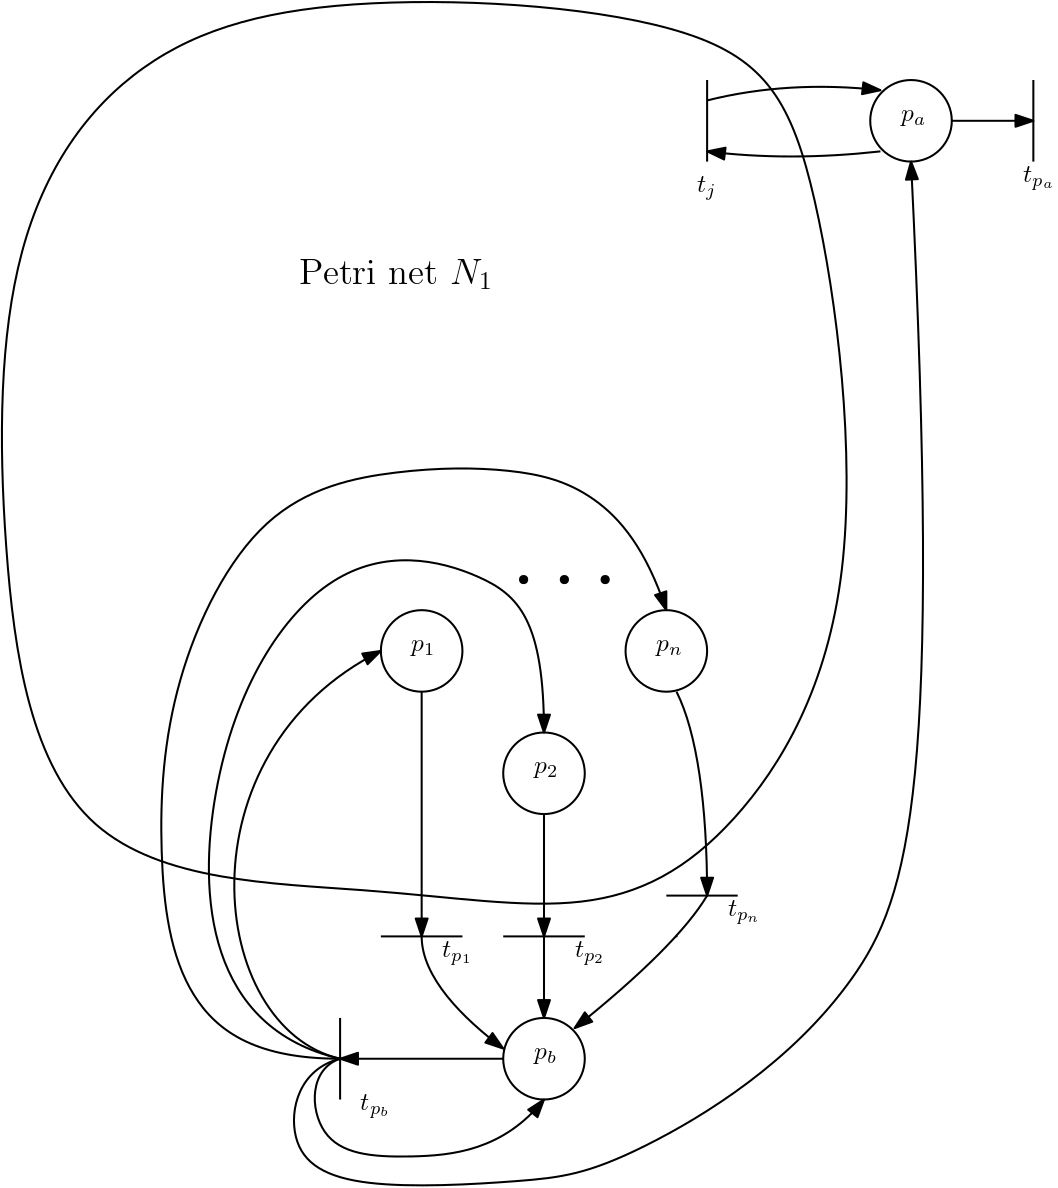
\includegraphics[width=0.75\textwidth]{FigurePN}
\caption{Construction of $N_2$ from $N_1$.}
	\end{figure}
\end{center}

Let us now prove that $t_{p_2}$ is live in $N_2$ if and only if 
the zero marking
is not reachable from $\mu_1$ in $N_1$. \\


{\bf Suppose that the zero marking is reachable from $\mu_1$ in $N_1$, then $t_{p_2}$ is not live in $N_2$}.

Indeed the marking with zero in every place of $P_1$ and in $p_b$ is reachable in $N_2$, by executing the same sequence of transition firings. Then $t_{p_a}$ can fire, leading to the marking which assigns zero to every place of $P_2$. From this marking the transitions $t_p$ are not live and neither are the transitions inherited from $N_1$ nor $t_{p_a}$, and, finally, nor is $t_{p_2}$. Thus $t_{p_2}$ is not live in $N_2$. \\


{\bf Suppose that $t_{p_2}$ is not live in $N_2$, then the zero marking is reachable from $\mu_1$ in $N_1$}

Indeed, if $t_{p_2}$ is not live in $N_2$, then a marking $\mu$ must be reachable in which $\mu(p_2) = 0$ and there is no reachable state in which $p_2$ has a token (in particular, since we do not allow token removal from $p_2$, the marking $\mu$ must be reached in a sequence of transitions that do not place any token in $p_2$).
This means that no transition $t_p$ is live in $N_2$ in $\mu$ since any transition $t_p$ can place a token in $p_2$. 
Thus, every place of $P_2$ inherited from $N_1$ must be devoid of token. Moreover, since the marking $\mu$ must be reached  in a sequence of transitions that do not place any token in $p_2$, 
it can be reached without using the transitions $t_p$ or $t_{p_2}$. Since $t_{p_a}$ do not modify the places inherited from $P_1$ nor does it enable new transitions, the reachability of $\mu$ implies the reachability of a marking where every place of $P_2$ inherited from $P_1$ is devoid of token using only the transitions inherited from $N_1$. Thus the zero marking is reachable from $\mu_1$ in $N_1$.
\end{proof}











\end{document}















